\chapter{DISCUSSION}

In this work, genome-scale metabolic modelling methods are used to analyze transcriptomics of evolved \emph{S. cerevisiae} strains that have obtained by in vivo evolutionary engineering strategies for different environmental conditions where the following substances are gradually increased in the media: Ethanol, caffeine, coniferylaldehyde, iron, nickel, phenylethanol, and silver.

Turanlı-Yıldız et. al., obtained two evolved clones that could tolerate up to 12\% (v/v) ethanol, namely B2 and B8 strains, under increasing ethanol levels \cite{TuranlYldz2017}. Apart from the important findings on triggered diploidization during adaptation, their transcriptome analyses revealed that the most enriched genes were related to carbohydrates storage metabolism, however, only B2 strain alone exhibited a higher glycogen accumulation. They have also found that the abundances of mitochondrial proteins were decreased in B8 strain, suggesting a reduced respiratory activity. On top of that, findings on higher abundances of ribosomal proteins, amino acid metabolism, and glycolysis supported the idea of a higher fermentation levels.

In silico simulations show that, under the same environmental conditions provided, B2 strain is able to grow at slightly higher rates compared to B8 strain, 0.347 h\textsuperscript{-1} and 0.337 h\textsuperscript{-1} respectively, while B8 strain is able to produce ethanol at a higher rate 10.667 mmol/gDWh\textsuperscript{-1} compared to 9.934 mmol/gDWh\textsuperscript{-1} for B2 strain. The main difference observed in simulations between B2 and B8 strains is the regulation of citrate in the TCA cycle, specifically the transport reaction,
\begin{align}
\label{eq:citratetransport}
\ citrate_c + isocitrate_m \xleftrightarrow[\text{Rev: B8 (0.319 mmol/gDWh\textsuperscript{-1})}]{\text{Fwd: B2 (0.218 mmol/gDWh\textsuperscript{-1})}} citrate_m + isocitrate_c
\end{align}
\noindent where the indicators \emph{c} is for the cytoplasmic, and \emph{m} is for the mitochondrial metabolites. Transportation of citrate from mitochondria to cytoplasm in B8 strain agrees with the experimental findings on the idea of reduced respiratory activity, and this idea is supported with the ferrocytochrome-c:oxygen oxidoreductase (oxidative phosphorilation) fluxes where B2 strain has higher flux rate 18.867 mmol/gDWh\textsuperscript{-1}, compared to 17.439 mmol/gDWh\textsuperscript{-1} on B8 strain.

Although there is not a clear indicator on the glycogen synthase on simulations, the reason behind a slightly higher growth rate for B2 strain could arise from the carbohydrate pseudoreaction (Equation \ref{eq:carbohydratepseudo}) required for biomass. However, it must be noted that only 0.003 mmol/gDWh\textsuperscript{-1} difference is observet between B2 and B8 clones for the glycogen (starch) synthase reaction where UDP-D-glucose is converted into glycogen.
\begin{align}
\begin{split}
\label{eq:carbohydratepseudo}
\  0.74851 \text{ (1-3)-beta-D-glucan} + 0.25009 \text{ (1-6)-beta-D-glucan } + \\
\ 0.36141 \text{ glycogen} + 0.71094 \text{ mannan} + 0.13828 \text{ trehalose} \xrightarrow{}  \text{carbohydrate}
\end{split}
\end{align}

Sürmeli et. al., obtained yeast populations that can survive at high caffeine levels \cite{Srmeli2019}. Contrary to expectations from literature, their evolved strain, Caf905-2, did not show any inhibitory efects on the growth during stress selection. Transcriptome analysis on the obtained evolved strain, showed that Cytochrome c isoform 2 (CYC7) was the most upregulated gene. It is known that CYC7 is an electron carrier of the mitochondrial intermembrane space, and it is expressed under hypoxic conditions. In our simulations, we were able to catch the over-expression of CYC7 on flux variability analysis (Table \ref{table:fva_results}). Caffeine resistant model reaches to highest growth rate among evolved strains, and it was able to maintain energy without oxidative phosphorylation. As it can be seen from the phenotype phase planes in Figure \ref{fig:robustness_glu_oxy}, caffeine resistant model is highly sensitive oxygen availability and cannot grow if the oxygen uptake rate is higher than 25 mmol/gDWh\textsuperscript{-1}. Flux balance analysis shows that caffeine resistant model reaches its maximum available growth rate of 0.468 h\textsuperscript{-1} when the oxygen uptake rate is 0.235 mmol/gDWh\textsuperscript{-1}. In other words, the model choses not to take oxygen from outside if the carbon supply is unlimited in the media, it simulates hypoxic conditios for best outcome. However, if the glucose uptake is forced to 10 mmol/gDWh\textsuperscript{-1}, model takes more oxygen at the rate 4.757 mmol/gDWh\textsuperscript{-1}.

In their work, it has also been reported the induction of genes involved in glycogen and trehalose metabolism under cafeine stress. However, since the genome-scale modelling does not simulate stress conditions (i.e., no caffeine molecule is provided into the defined medium), this finding is not observed in the simulations, suggesting that this change could be regulated on the metabolic level, not on the transcriptomics level. Additionally, upregulation of SNQ2 was also not captured in the simulations, due to lack of its gene association in the Yeast8 model.

Transcriptomic changes in a coniferylaldehyde resistant yeast population, BH13, is reported by Hacısalihoğlu et. al., and differential regulations after adaptive evolution on the NAD(P)-dependent aldehyde dehydrogenases are revealed. They reported that all members of aldehyde dehydrogenases (ALD) except for ALD5 were upregulated, and ALD upregulation were previously observed in the literature \cite{adeboye2015catabolism}. Additionally, oxidoreductase enzymes such as BDH2, YPL113C, YJR096W; and putative aryl-alcohol dehydrogenases such as YPL088W and AAD15 were reported as upregulated in coniferylaldehyde resistant strain. Here, in flux variability analysis, ALD4 upregulation is observed in coniferylaldehyde resistant model, accompanied with the caffeine and phenylethanol resistant strains. From the experimental findings, cross-resistance were reported for the caffeine resistant strain for coniferylaldehyde stress, and a coniferylaldehyde resistant strain was also cross-resistant to cafeine stress. Considering this, our findings suggest that phenylethanol resistant strain may show a similar cross-resistance (experimental data on phenylethanol resistant strain is not published yet), and ALD gene family should be investigated in more detail. It is also observed that only these three (caffeine, coniferylaldehyde, and phenylethanol) models do not carry fluxes through fatty acid metabolism when the flux variability results are investigated pathway-wise.

In the coniferylaldehyde resistant strain, Hacısalihoğlu et. al. reported that the glucose uptake and metabolism were enhanced even without the coniferylaldehyde stress in the media \cite{Hacsaliholu2019}. This observation is explained by the upregulation of the genes encoding hexose transporters, and the enzymes involved in glycolysis, namely HXK1, GLK1, TDH1, GPM2, ERR1, and PYK2. Increased glucose uptake compared to wild-type model, and high flux range on flux variability analysis for HXK1, GLK1, and PYK2 in coniferylaldehyde resistant model confirms in silico simulations to the experimental findings. Similar to the results of ADL family, GLK1 enzyme has a higher flux range in caffeine and phenylethanol resistant models next to coniferylaldehyde resistant model. Interestingly, for the flux range of PYK2, iron resistant model accompanies coniferylaldehyde and caffeine resistant models instead of phenylethanol resistant model.


Iron resistant \emph{S. cerevisiae} mutant, M8FE, is obtained by Balaban et. al with cross resistance feature to other metals \cite{balaban2020evolutionary}, and their findings suggested that the resistance to the metals might be related to the downregulation of PHO84 gene, encoding a high-affinity inorganic phosphate transporter and also a low-affinity manganese transporter. Unfortunately, phosphate uptake rates show no significant difference on in silico simulations. In the experiments, it is assumed that high amounts of iron would lead to oxidative stress that damage the cells, however, ROS amounts of the evolved M8FE strain were lower compared to reference strain. This phenomena explained with the microarray results, where the upregulation on the oxidative stress response genes were observed. This upregulation is assumed to achieved in order to reduce oxidative levels in the cell. In the simulations, iron resistant model was able to grow at the same rate with the wildtype model when the maximum glucose uptake is allowed (Table \ref{table:growth_glucose_table}). However, when we consider ATP production, despite having high glucose uptake and growth rates as wildtype model, iron resistant model has much lower fluxes through ATP producing reactions compared to other models (Figure \ref{fig:fba_gro_glu_atp}). Although there is no in silico confirmation, Balaban et. al. suggests that the iron resistant strain prefers to save its energy as trehalose in the cell.

Their study also reported upregulations on the glycogen phosphorylase gene, GPH1; and phosphoglucomutase, PGM2. Here, flux variability analyses showed a high range for all evolved models for the enzyme PGM2, catalyst of the conversion from glucose-1-phosphate to glucose-6-phosphate, except in the silver resistant model. That being said, the upregulation in the PGM2 might possibly be related to DNA replication stress, and not a specific upregulation for the metal stress.



\subsection{Glyceraldehyde-3-phosphate dehydrogenase}
The most divergent enzyme through all evolved model simulations, glyceraldehyde-3-phosphate dehydrogenase (GAPDH) is an enzyme involved in glycolysis and gluconeogenesis pathways and it is encoded by three genes TDH1, TDH2 and TDH3 (triose-phosphate dehydrogenase; TDH) \cite{boucherie1995differential}. It catalyses the conversion of glyceraldehyde-3-phosphate to 1,3-bisphospho-D-glycerate during glycolysis and the reverse reaction during gluconeogenesis (Eq. \ref{eq:GAPDH}).
\begin{align}
\label{eq:GAPDH}
\begin{split}
\ \text{glyceraldehyde-3-phosphate} + NAD + P \leftrightarrow \\
\ \text{1,3-bisphospho-D-glycerate} + H^+ + NADH
\end{split}
\end{align}
In this study, it is found that carried flux through GAPDH is increased by 39\% in caffeine, 13\% in silver, and 11\% in coniferylaldehyde resistant model. On the contrary, the carried flux is decreased by 31\% in ethanolb2, 15\% in ethanolb8, and 26\% in iron resistant model. It is also observed that each evolved model uses different isozyme for the catalytic activity. GAPDH differences are summarized in Figure \ref{fig:discuss_GAPDH}.

For a long time, GAPDH was considered as an housekeeping gene for its constitutively expression in the cell, and commonly used in comparisons of expression data. In 2005, Barber et al. have reported different regulation mechanisms for GAPDH under specific conditions\cite{barber2005gapdh}, and it is later found that the gene is upregulated under hypoxic stress \cite{yang2008effects}. Additional functions in other cellular processes has also been described such as being a chaperone protein in cellular iron homeostasis \cite{sweeny2018glyceraldehyde}. Interestingly, catalytically active TDH enzymes are found in both the cytoplasm and the cell wall.

\begin{figure}[H]
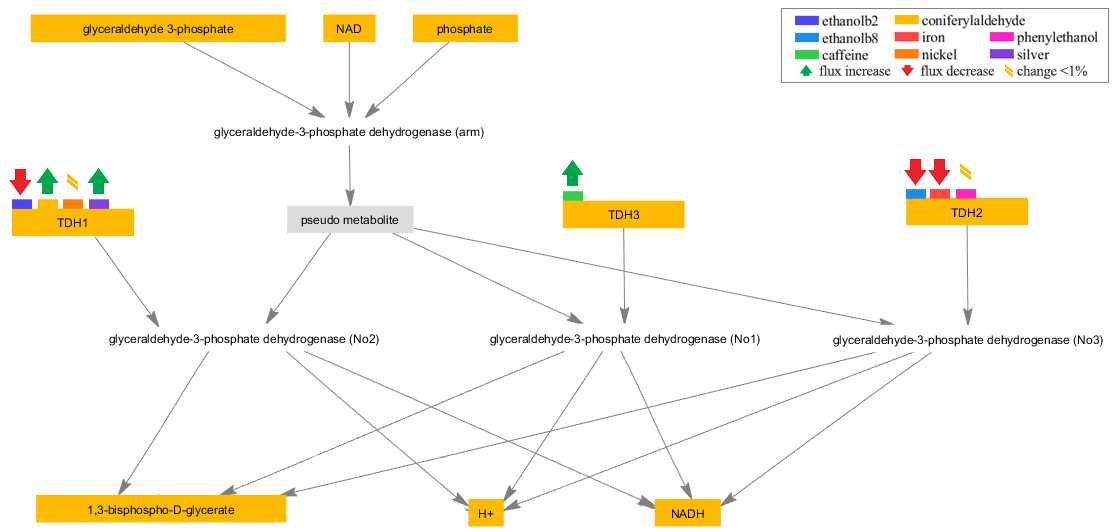
\includegraphics[width=1\columnwidth]{figures/discuss_GAPDH.png}
\caption[Map of glyceraldehyde-3-phosphate dehydrogenase catalized reaction as it used in simulations]{Map of glyceraldehyde-3-phosphate dehydrogenase catalized reaction as it used in simulations. Corresponding genes used for evolved models are shown in colors, and flux changes from wildtype model simulations are indicated as increased or decreased with arrows.}
\label{fig:discuss_GAPDH}
\end{figure}

GAPDH activity is controlled with oxygen availability, and evidence suggests that it may be the sensor of the cell in terms of oxidative stress \cite{chuang2005glyceraldehyde}. In the simulations presented here, oxidative phosphorylation through ATP synthase was totally inactive (zero flux) for the caffeine resistant model under unconstrained conditions, i.e., unlimited availability for uptake metabolites such as oxygen and glucose. Despite the inactivity, caffeine resistant model was the highest ATP producer among evolved models, and the ATP production was through pyruvate kinase and phosphoglycerate kinase activies (Table \ref{table:fba_atp_production}). Similar to caffeine resistant model, silver resistant model, too, showed increased activity on GAPDH and carried zero flux through ATP synthase in oxidative phosphorylation. In agreement with the results, ethanholb2, ethanolb8, and iron resistant models showed decreased activity for GAPDH and they were the only models that show ATP synthase activity.
